\chapter{Теоретико-аналитическая часть}

  \section{Постановка задачи}

    Исследовать возможность использования семантико-синтаксического
    анализатора Compreno в качестве источника высокоуровневых признаков для задачи
    NER на корпусе CoNLL 2003 в рамках нейросетевого подхода.

  \section{Обзор литературы}

    Победители соревнования по NER CoNLL 2003 \citep{florian2003named}, получившие 88.76\% F1,
    представили систему использующую комбинацию различных алгоритмов машинного обучения.
    В качестве признаков был использован их собственный, вручную составленный газетир,
    POS-теги, CHUNK-теги, суффиксы, префиксы и выход других NER-классификаторов,
    тренированных на внешних данных.

    \citep{collobert2011natural} представили комбинацию сверточной нейронной сети
    с условными случайными полями, получившую 89.59\% F1 на корпусе CoNLL 2003.
    Их нейросетевая архитектура не зависит от задачи и используется как для NER, так и для
    частеречной разметки (part-of-speech tagging), поиска синтаксически связанных групп
    соседних слов (chunking), установления семантических ролей (semantic role labelling).
    Для задачи NER они использовали три типа признаков - векторное представление слова,
    капитализацию и небольшой газетир, включенный в соревнование CoNLL 2003.

    \citep{chiu2015named} представили комбинацию сверточных сетей, рекуррентных сетей
    и условных случайных полей показывающую 91.62\% F1.
    Они использовали такие же признаки как у \citep{collobert2011natural}, дополнительный, вручную сформированный
    газетир на основе DBpedia и обучались на
    train+dev\footnote{Объединенная обучающая и валидационная выборки} выборке CoNLL 2003.
    Кроме корпуса CoNLL 2003 они тестировали архитектуру
    на более крупном англоязычном корпусе OntoNotes 5.0. На нем они получили
    state-of-the-art результат 86.28\%.

    \citep{DBLP:journals/corr/YangSC16} представили глубокую иерархическую рекуррентную нейросетевую
    архитектуру с условными случайными полями для разметки последовательностей.
    Они использовали такие же признаки как у \citep{collobert2011natural}.
    Кроме англоязычного корпуса CoNLL 2003, где они получили state-of-the-art 90.94\% F1 при обучении
    только на обучающей выборке (train set), они тестировали работу нейросети на CoNLL 2002 Dutch NER и CoNLL 2003 Spanish NER.
    На этих корпусах они улучшили предыдущий state-of-the-art результат:
    82.82\% до 85.19\% на CoNLL 2002 Dutch NER и 85.75\% до 85.77\% на CoNLL 2003 Spanish NER.

    Современные работы используют векторное представление слов
    и условные случайные поля в своих моделях. Из сторонних признаков применяют
    только газетиры. В работах \citep{xu2014rc, bian2014knowledge} описано применение дополнительных признаков для
    слов (морфологических, синтаксических, семантических) для создания более
    совершенных векторных представлений.
    Такие векторные представления помогают повысить оценку качества в
    прикладных задачах \citep{xu2014rc}.

  \section{Обзор корпуса CoNLL 2003}

  В данной работе рассмотрен англоязычный корпус CoNLL 2003, т.к. он является
  одним из самых распространенных корпусов на котором год от года измеряют оценку качества
  методов распознавания именованных сущностей.

  CoNLL 2003 \citep{tjong2003introduction} - англоязычный корпус для оценки качества
  методов распознавания именованных сущностей.
  Корпус содержит обучающую, тестовую и валидационную выборку.
  Размечено 4 типа сущностей - персоны (PER), организации (ORG), локации (LOC) и другие (MISC).
  \newpage
  \begin{table}[!h]
    \caption{Количество статей, предложений, токенов и именованных сущностей}
    \centering
    \begin{tabular}{ | p{2.9cm} | p{1.5cm} | p{2.5cm} | p{1.5cm} | p{1cm} | p{1.1cm} | p{1cm}| p{1cm} |}
      \hline\hline
      Выборка & Статьи & Предлож-я & Токены & LOC & MISC & ORG & PER \\
      \hline
      Обучающая & 946 & 14987 & 203621 & 7140 & 3438 & 6321 & 6600 \\
      \hline
      Валидац-я & 216 & 3466 & 51362 & 1837 & 922 & 1341 & 1842 \\
      \hline
      Тестовая & 231 & 3684 & 46435 & 1668 & 702 & 1661 & 1617 \\
      \hline
    \end{tabular}
  \end{table}

  Корпус размечен по схеме \textit{Inside, Outside, Begin (IOB)}:
  \begin{itemize}
  \item слово помечают тегом O (Outside), если оно не является именованной сущностью.
  \item Тегом I-XXX (Inside), где XXX - тип именованной сущности, если слово
    является именованной сущности или ее частью.
  \item Тегом B-XXX (Begin), если слово является началом именованной сущности.
  \end{itemize}

  Пример:
  \centerline{}
  \centerline{, O}
  \centerline{Surrey I-ORG}
  \centerline{captain O}
  \centerline{Chris B-PER}
  \centerline{Lewis I-PER}
  \centerline{, O}

  Оценка качества считается с помощью метрики $F_{\beta=1}$(F1-micro-average):
  \[
    F_\beta = \frac{(\beta^2 + 1) * precision * recall}{\beta^2*precision + recall},
  \]
  где $precision$ (точность) - процент корректных именованных сущностей
  найденных системой, $recall$ (полнота) - процент всех именованных сущностей
  найденных системой. Именованная сущность считается найденной корректно, если
  вся сущность помечена правильно.
  В CoNLL 2003 включен скрипт conlleval, оценивающий качество классификации.

  В работе \citep{collobert2011natural} предлагается использовать схему
  \textit{Inside, Outside, Begin, End, Single (IOBES)}, т.к. она более явно указывает
  тег для слова:
  \begin{itemize}
  \item слово помечают тегом O (Outside), если оно не является именованной сущностью.
  \item Тегом I-XXX (Inside), где XXX - тип именованной сущности, если слово является частью именованной сущности.
  \item Тегом B-XXX (Begin), если слово является началом именованной сущности.
  \item Тегом E-XXX (End), если слово является концом именованной сущности.
  \item Тегом S-XXX (Single), если именованная сущность состоит из одного слова.
  \end{itemize}

  Пример:
  \centerline{}
  \centerline{, O}
  \centerline{Surrey S-ORG}
  \centerline{captain O}
  \centerline{Chris B-PER}
  \centerline{Lewis E-PER}
  \centerline{, O}

  Во время оценки качества, IOBES конвертируют в IOB и подают на вход conlleval.

  Также в CoNLL 2003 включен небольшой газетир.

  \section{Обзор нейросетевого подхода к решению задачи NER}  \label{section:nn}

  Традиционным подходом к решению задач из области автоматической обработки текстов,
  включая NER, является использованием алгоритма обучения с учителем, например
  машины опорных векторов с линейным ядром. Вручную составленные признаки подаются на вход
  алгоритма обучения с учителем. Выбор признаков - это практически полностью эмпирический
  процесс, построенный на лингвистической интуиции и решаемой задаче.

  Нейросетевой подход предполагает использование минимального количества признаков.
  Обычно это векторные представления слов полученные из большого корпуса с использованием
  алгоритмов обучения без учителя.

  В этом разделе будет рассмотрен нейросетевой подход из работы
  \citep{collobert2011natural}. Была выбрана именно эта работа так как:
  \begin{itemize}
  \item в ней представлена модель, получающая сравнимую со state-of-the-art F1-меру на CoNLL 2003,
  \item представленная модель имеет различные программные имплементации,
  \item векторные представления слов под названием <<Senna Embeddings>>
    используемые в этой работе находятся в открытом доступе в сети.
  \end{itemize}
  Последние два пункта указывают на возможность воспроизведения результатов из статьи относительно небольшими усилиями.

  \subsection{Векторные представления слов}

  Согласно Википедии\footnote{\url{https://en.wikipedia.org/wiki/Word_embedding}},
  \textit{векторное представление} — это общее название для различных
  подходов к моделированию языка и обучению представлений в обработке естественного языка,
  направленных на сопоставление словам (и, возможно, фразам) из некоторого словаря $D$,
  векторов из $R^n$, где $n$ - значительно меньше $|D|$ (обычно от 50 до 1000).

  \citep{collobert2011natural} использовали нейронные сети для построения векторных представлений слов.
  Они тренировали нейронную сеть на данных корпуса английской
  Википедии\footnote{На данных ноября 2007 года из http://download.wikimedia.org}
  и Reuters RCV1\footnote{Доступно http://trec.nist.gov/data/reuters/reuters.html}.
  Были использованы 130000 самых частотных слов, остальные слова кодировались
  специальным токеном UNKNOWN.
  Полученные векторные представления называются Senna Embeddings и доступны в сети
  по адресу: http://ronan.collobert.com/senna/.

  Senna Embeddings использовались как входные признаки на нейронные сети для решения задачи NER.

  \subsection{Описание нейросетевых моделей} \label{subsection:nn}

  В работе \citep{collobert2011natural} описываются две нейросетевые модели:
  \begin{itemize}
  \item оконный (window), который предсказывает тег слова на основе контекста (окна) вокруг слова,
  \item сверточный (convolution), который предсказывает тег слова используя всё предложение.
  \end{itemize}

  \subsubsection{Оконная модель} \label{subsubsection:window}
  Оконная модель представлена на рис. \ref{figure:window_net}.
  \newpage
  \begin{figure}[!h]
    \centering
    \caption{Оконная модель из \citep{collobert2011natural}}
    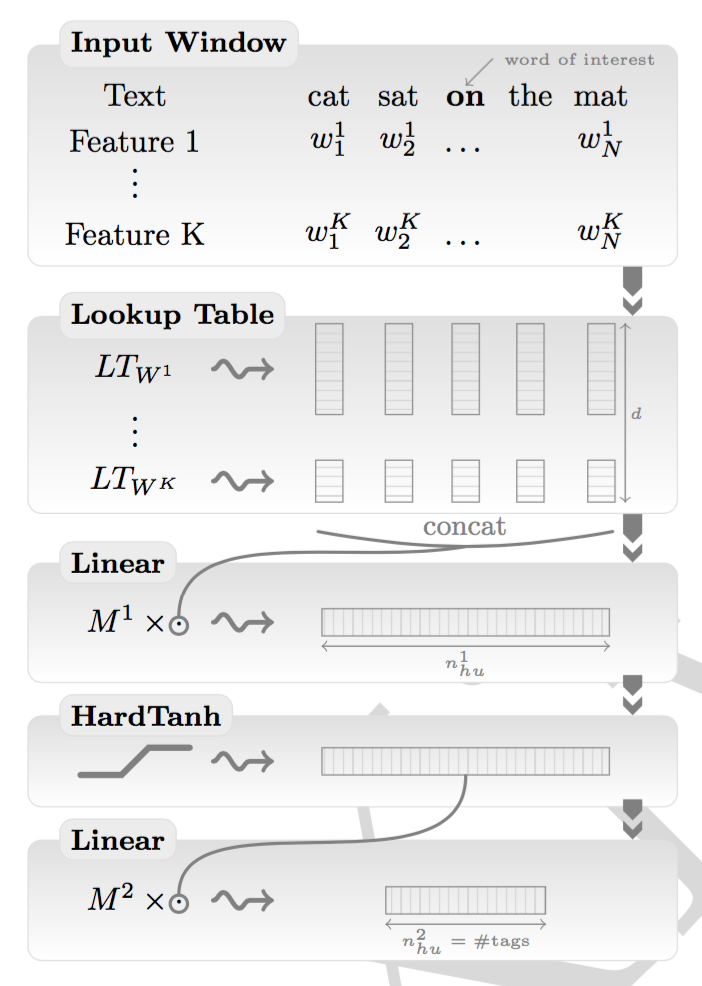
\includegraphics{figures/window.png}
    \label{figure:window_net}
  \end{figure}

  На рис. \ref{figure:window_net} предсказывается тег для слова on.
  При классификации используется контекст для этого слова.
  Всё окно состоящее из 5 слов пропускается через так называемый Lookup Table.

  \textit{Lookup Table} - это специальной слой в нейронной сети, который
  отображает каждое слово в вектор весов. Причем вектор весов обучается вместе с сетью.
  Более формально, каждому слову $w$ из словаря $D$ ставится в соответствие
  вектор размерности $d$, который задается Lookup Table слоем $LT_W(w)$:
  \[
    LT_W(w) = W_{\cdot,w},
  \]
  где $W \in R^{d\times|D|}$ - матрица весов для обучения, $W_{\cdot,w}$ - $w$-ый столбец
  матрицы $W$. Размерность $d$ - гиперпараметр.

  Также этот слой может принимать на вход последовательность слов $w_1 \ldots w_K$,
  где $K$ - величина окна. В этом случае выходом будет матрица:
  \[
    f_1 = LT_W(w_1 \ldots w_K) = ( W_{\cdot, w_1} \ldots W_{\cdot, w_K})
  \]

  После Lookup Table слоя, полученная матрица преобразуется в один вектор с
  помощью операции \textit{конкатенации (Concat)}:
  \[
    f_{2} = Concat(LT_W(w_1 \ldots w_K)) =
      \begin{bmatrix}
        W_{\cdot, w_1} \\
        \vdots \\
        W_{\cdot, w_K}
      \end{bmatrix},
  \]

  Затем этот вектор подается на \textit{полносвязный слой (Linear Layer)}, который
  выполняет аффинное преобразование:
  \begin{equation} \label{formula:linear_layer}
    f_{3} = Linear(f_{2}) = W^2 f_{2} + b^2,
  \end{equation}
  где $W^2 \in R^{d_{2} \times |f_{2}|}$, $b \in R^{d_2}$. Гиперпараметр $d_{2}$ -
  это количество нейронов в данном слое.

  Каждый элемент полученного вектора $f_3 \in R^{d_2}$ пропускается через нелинейную функцию.
  На рис. \ref{figure:window_net} это \textit{HardTanh}:
  \[
    f_{4} = HardTanh(f_{3}),
  \]
  \begin{equation} \label{formula:hard_tanh}
  HardTanh(x) =
    \begin{cases}
      -1, \text{if } x < -1 \\
      x, \text{if } -1 <= x <= 1 \\
      1, \text{if } x > 1
    \end{cases}
  \end{equation}
  Преимуществом этой функции перед гиперболическим тангенсом является более быстрое
  время вычисления.

  Последний слоем является полносвязный слой. Количество нейронов в нем
  равно количеству предсказываемых классов.
  \[
    f_5 = Linear(f_4) = W^5 f_{4} + b^5.
  \]

  Каждый элемент $x_i$ полученного вектора $f_5$ пропускается через функцию \textit{Softmax} для получения
  вероятностей:
  \[
    Softmax(x_{i}) = \frac{e^{x_{i}}}{\sum_j e^{x_{j}}}
  \]
  Другими словами это нормализация вектора с помощью экспоненциальной функции.

  Для обучения нейронной сети минимизируется функционал ошибки с использованием
  пакетного градиентного спуска (mini-batch gradient descent).
  \textit{Функционал ошибки $C$}:
  \[
    C = - \sum_{(x, y_k) \in T} \log(\Prob(y_k | x, \theta)),
  \]
  \[
    C \rightarrow \min_\theta,
  \]
  \[
    \log(\Prob(y_k | x, \theta)) = f_4(y_k) - \log\sum_i e^{f_4(y_i)},
  \]
  где $(x, y_k)$ - пара объект, класс из обучающей выборки $T$; $\theta$ - веса
  всей нейросети (все матрицы $W$), $f_4(y_i)$ - значение последнего слоя для класса $y_i$.

  Функционал ошибки $C$ минимизируется с помощью \textit{пакетного градиентного спуска}:
  \[
    \theta = \theta - \alpha\sum_{(x, y_k) \in T_s}\nabla_{\theta}(-\log\Prob(y_k | x, \theta)),
  \]
  где $\alpha$ - шаг обучения, $T_s$ - случайное подмножество объектов из обучающей выборки.
  Размер подмножества $T_s$ и $\alpha$ являются гиперпараметрами.

  \textit{Стохастический градиентный спуск (stochastic gradient descent)} является
  модификацией пакетного градиентного спуска. Отличие заключается в том, что размер $T_s$ равен 1.

  \subsubsection{Сверточная модель}  \label{subsubsection:conv}
  Сверточная модель представлена на рис. \ref{figure:conv_net}.
  \newpage
  \begin{figure}[!h]
    \centering
    \caption{Сверточная модель из \citep{collobert2011natural}}
    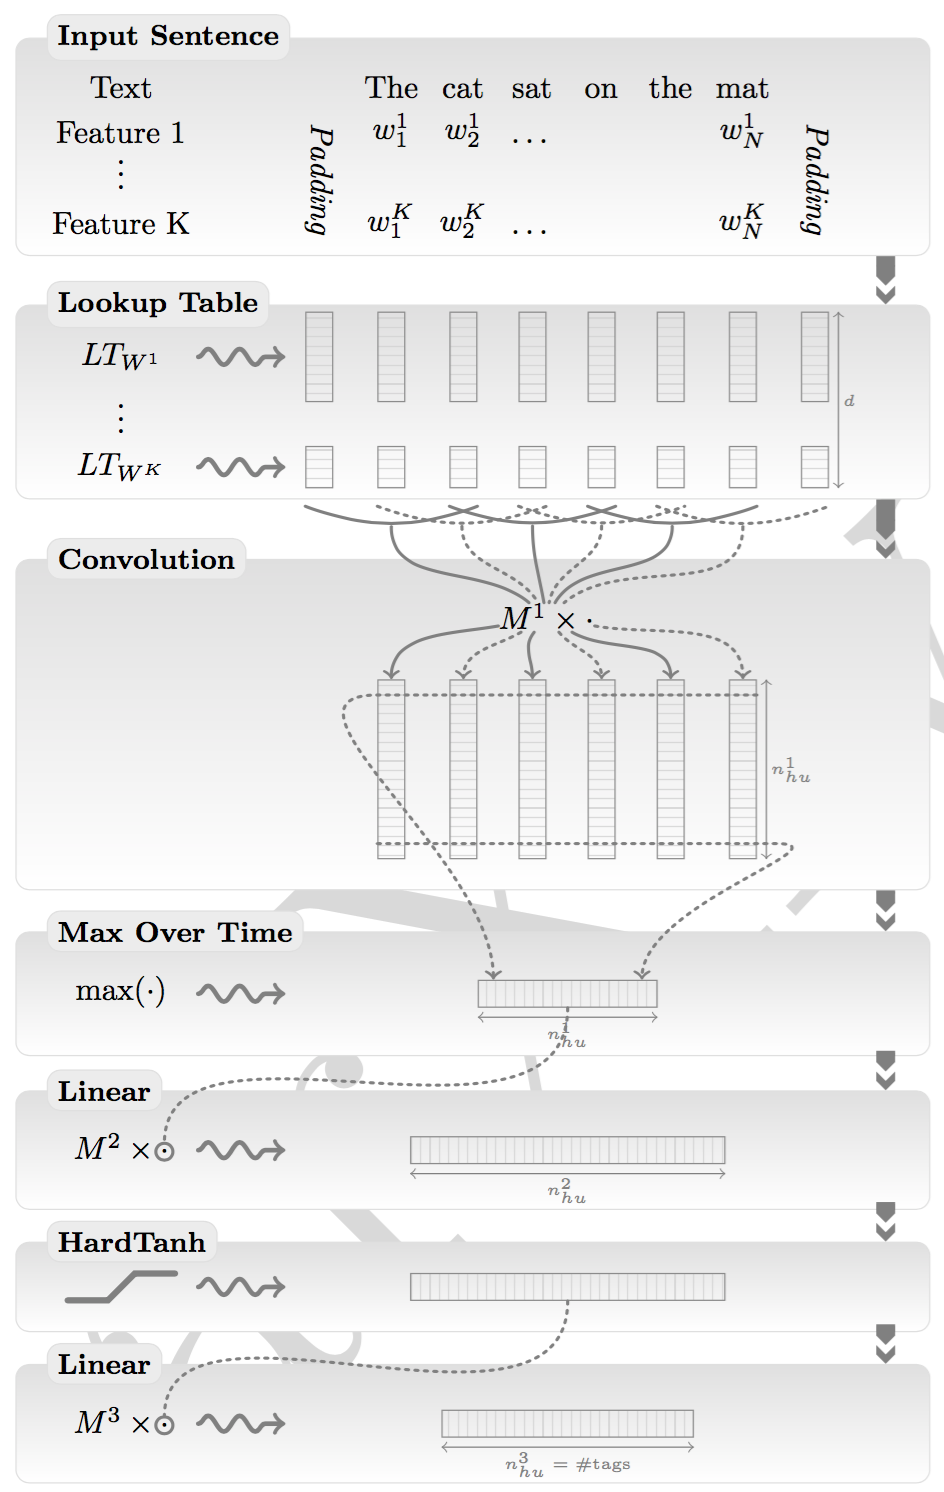
\includegraphics[scale=0.9]{figures/sentence-diagram.png}
    \label{figure:conv_net}
  \end{figure}

  В отличие от оконной модели, она принимает на вход всё предложение.

  Все слова предложения пропускаются через Lookup Table, как описано в разделе
  \ref{subsubsection:window}, после чего попадают на сверточный слой.

  \textit{Сверточный слой (temporal convolution)} является обобщением
  полносвязного слоя (\ref{formula:linear_layer}) из оконного подхода:
  \begin{enumerate}
    \item сначала осуществляется проход окном на полученной на предыдущем шаге матрице $f_1$,
    \item столбцы попавшие в окно конкатенируются,
    \item полученный вектор пропускается через полносвязный слой,
    причем матрица весов $W^3$ является одной и той же в каждом проходе.
  \end{enumerate}
  На выходе, после прохода окном по всей матрице $f_1$, получается матрица $f_3$.
  Более формально:
  \[
  f_3 =(W^3 f_1[1, d_{win}] + b^3,\ldots,W^3 f_1[|f_1| - d_{win}, d_{win}] + b^3),
  \]
  \[
  d_{f_1, win} = d_{win}*d,
  \]
  где $f_1[i, d_{win}]$ - означает конкатенацию столбцов $f_1$ с $i$ по $i + d_{win}$,
  $d_{f_1, win}$ - размерность полученного после конкатенации вектора $f_1[i, d_{win}]$,
  $W^3 \in R^{d_{2} \times d_{f_1, win}}$, $b \in R^{d_2}$. Гиперпараметр $d_{2}$ -
  это количество нейронов в данном слое.

  После того как всё предложение прошло через Lookup Table и сверточный слой
  получается матрица $f_3 \in R^{d_2\times |f_1| - d_{win}}$.
  Количество строк в ней фиксировано, но количество столбцов зависит от длины предложения.
  Чтобы получить вектор признаков фиксированный длины выполняется \textit{операция
  получения максимума по строкам (Max over time)} над $f_3$.
  Смысл этой операции заключается в получении наиболее значимых признаков из каждого окна.
  Из каждой строки матрицы $f_3$ извлекается максимум и в результате этой
  операции получается вектор $f_5 \in R^{d_2}$.

  Далее над полученным фиксированным вектором признаков проводятся уже
  знакомые по разделу \ref{subsubsection:window}
  операции с полносвязными слоями (\ref{formula:linear_layer}) и
  нелинейной функцией HardTanh (\ref{formula:hard_tanh}).

  Для обучения используется минимизация функционала ошибки и пакетный градиентный
  спуск описанные в разделе \ref{subsubsection:window}.

  В оригинальное статье \citep{collobert2011natural} в сверточном подходе
  минимизировался другой функционал ошибки, который включает в себя условные случайные поля.
  Это позволило им достичь более высокой оценки качества, но в то же время замедлило
  время проведения экспериментов. Данный функционал не поддерживается библиотеками для
  работы с нейронными сетями, поэтому его необходимо реализовывать с нуля.
  Из-за этих причин этот функционал ошибки не рассмотрен в этой работе.

  \subsubsection{Уточнения к моделям}

  В разделе \ref{subsubsection:conv} теги предсказываются для каждого слова.
  Т.к. на вход нейросети поступает предложение, то необходимо кодировать
  местоположение слова в предложении для которого предсказывается тег.
  Это осуществлялось с помощью Lookup Table.
  Позиция слова $w_j$ в предложении кодировалась
  с помощью подсчета расстояния относительно слова $w_i$ для которого предсказывается тег.
  Слово $w_i$ кодировалось в Lookup Table как $0$. Слово $w_{i-k}$ как $-k$. Слово $w_{i+k}$ как $+k$.

  В качестве регуляризации использовался Dropout слой после каждого полносвязного слоя,
  кроме последнего.
  Dropout слой \citep{srivastava2014dropout} с заданной вероятностью $p$ зануляет
  выход нейрона.

  Важным условием хорошего обучения нейронной сети является начальная инициализация
  весов. В данной работе использовано 2 подхода к инициализации весов:
  \begin{enumerate}
  \item $U(\frac{-1}{\sqrt{fi}}, \frac{1}{\sqrt{fi}})$
  \item $U(-\sqrt{\frac{2}{fi + fo}}, \sqrt{\frac{2}{fi + fo}}),$
  \end{enumerate}
  где $U$ - равномерное распределение, $fi$ - количество входов в слой,
  $fo$ - количество выходов из слоя.
  Первый подход описан в \citep{collobert2011natural}, второй в \citep{glorot2010understanding}.


  \section{Обзор синтактико-семантических признаков}
    Существует много инструментов для получения дополнительных признаков для слова.
    Для извлечения синтаксических признаков часто используют MaltParser \citep{nivre2006maltparser}.
    Для получения семантических признаков применяют BabelNet \citep{navigli2010babelnet}.

    В данной работе для получения синтактико-семантических признаков используется Compreno.
    Признаки синтактико-семантического дерева Compreno кодировались в бинарные вектора
    и соотносились с токенами исходного
    текста\footnote{Почти для всех токенов в соответствующем дереве нашлась соответствующая вершина.
    Токены для которых не была найдена вершина, кодировались специальным признаком 83951},
    тем самым наделяя их синтактико-се\-ман\-ти\-ческими признаками.
    Размерность пространства синтактико-се\-ман\-ти\-ческих признаков получилась равной 83951.

    Плотные вектора большой размерности сильно замедляют процесс оптимизации и для хорошего
    обучения требуется много данных и вычислительных ресурсов.
    В таких случаях часто применяют методы для уменьшения размерности,
    например сингулярное разложение (SVD) или автоэнкодеры. Минусом таких методов является потеря информации
    после сжатия.

    Если же вектора большой размерности разреженные, то используют специальные методы для
    работы с такими данными \citep{davissurvey}.

    В данной работе предлагается 2 способа внедрения синтактико-семантических признаков:
    \begin{itemize}
      \item сжать синтактико-семантические вектора с помощью сингулярного разложения и добавить
      как еще один Lookup Table в сверточную нейронную сеть;
      \item добавить еще одну нейронную сеть для синтактико-семантических признаков и оптимизировать
      её вместе со сверточной нейронной сетью.
    \end{itemize}
